%%%%%%%%%%%%%%%%%%%%%%%%%%%%%%%%%%%%%%%%%
% Wenneker Article
% LaTeX Template
% Version 2.0 (28/2/17)
%
% This template was downloaded from:
% http://www.LaTeXTemplates.com
%
% Authors:
% Vel (vel@LaTeXTemplates.com)
% Frits Wenneker
%
% License:
% CC BY-NC-SA 3.0 (http://creativecommons.org/licenses/by-nc-sa/3.0/)
%
%%%%%%%%%%%%%%%%%%%%%%%%%%%%%%%%%%%%%%%%%

%----------------------------------------------------------------------------------------
%	PACKAGES AND OTHER DOCUMENT CONFIGURATIONS
%----------------------------------------------------------------------------------------

\documentclass[10pt, a4paper, twocolumn]{article} % 10pt font size (11 and 12 also possible), A4 paper (letterpaper for US letter) and two column layout (remove for one column)

%%%%%%%%%%%%%%%%%%%%%%%%%%%%%%%%%%%%%%%%%
% Wenneker Article
% Structure Specification File
% Version 1.0 (28/2/17)
%
% This file originates from:
% http://www.LaTeXTemplates.com
%
% Authors:
% Frits Wenneker
% Vel (vel@LaTeXTemplates.com)
%
% License:
% CC BY-NC-SA 3.0 (http://creativecommons.org/licenses/by-nc-sa/3.0/)
%
%%%%%%%%%%%%%%%%%%%%%%%%%%%%%%%%%%%%%%%%%

%----------------------------------------------------------------------------------------
%	PACKAGES AND OTHER DOCUMENT CONFIGURATIONS
%----------------------------------------------------------------------------------------

\usepackage[english]{babel} % English language hyphenation

\usepackage{microtype} % Better typography

\usepackage{amsmath,amsfonts,amsthm} % Math packages for equations

\usepackage[svgnames]{xcolor} % Enabling colors by their 'svgnames'

\usepackage[hang, small, labelfont=bf, up, textfont=it]{caption} % Custom captions under/above tables and figures

\usepackage{booktabs} % Horizontal rules in tables

\usepackage{lastpage} % Used to determine the number of pages in the document (for "Page X of Total")

\usepackage{graphicx} % Required for adding images

\usepackage{enumitem} % Required for customising lists
\setlist{noitemsep} % Remove spacing between bullet/numbered list elements

\usepackage{sectsty} % Enables custom section titles
\allsectionsfont{\usefont{OT1}{phv}{b}{n}} % Change the font of all section commands (Helvetica)

% MINE

\usepackage{amsmath}
\DeclareMathOperator*{\argmax}{arg\,max}
\DeclareMathOperator*{\argmin}{arg\,min}

%----------------------------------------------------------------------------------------
%	MARGINS AND SPACING
%----------------------------------------------------------------------------------------

\usepackage{geometry} % Required for adjusting page dimensions

\geometry{
	top=1cm, % Top margin
	bottom=1.5cm, % Bottom margin
	left=2cm, % Left margin
	right=2cm, % Right margin
	includehead, % Include space for a header
	includefoot, % Include space for a footer
	%showframe, % Uncomment to show how the type block is set on the page
}

\setlength{\columnsep}{7mm} % Column separation width

%----------------------------------------------------------------------------------------
%	FONTS
%----------------------------------------------------------------------------------------

\usepackage[T1]{fontenc} % Output font encoding for international characters
\usepackage[utf8]{inputenc} % Required for inputting international characters

\usepackage{XCharter} % Use the XCharter font

%----------------------------------------------------------------------------------------
%	HEADERS AND FOOTERS
%----------------------------------------------------------------------------------------

\usepackage{fancyhdr} % Needed to define custom headers/footers
\pagestyle{fancy} % Enables the custom headers/footers

\renewcommand{\headrulewidth}{0.0pt} % No header rule
\renewcommand{\footrulewidth}{0.4pt} % Thin footer rule

\renewcommand{\sectionmark}[1]{\markboth{#1}{}} % Removes the section number from the header when \leftmark is used

%\nouppercase\leftmark % Add this to one of the lines below if you want a section title in the header/footer

% Headers
\lhead{} % Left header
\chead{\textit{\thetitle}} % Center header - currently printing the article title
\rhead{} % Right header

% Footers
\lfoot{} % Left footer
\cfoot{} % Center footer
\rfoot{\footnotesize Page \thepage\ of \pageref{LastPage}} % Right footer, "Page 1 of 2"

\fancypagestyle{firstpage}{ % Page style for the first page with the title
	\fancyhf{}
	\renewcommand{\footrulewidth}{0pt} % Suppress footer rule
}

%----------------------------------------------------------------------------------------
%	TITLE SECTION
%----------------------------------------------------------------------------------------

\newcommand{\authorstyle}[1]{{\large\usefont{OT1}{phv}{b}{n}\color{DarkRed}#1}} % Authors style (Helvetica)

\newcommand{\institution}[1]{{\footnotesize\usefont{OT1}{phv}{m}{sl}\color{Black}#1}} % Institutions style (Helvetica)

\usepackage{titling} % Allows custom title configuration

\newcommand{\HorRule}{\color{DarkGoldenrod}\rule{\linewidth}{1pt}} % Defines the gold horizontal rule around the title

\pretitle{
	\vspace{-30pt} % Move the entire title section up
	\HorRule\vspace{10pt} % Horizontal rule before the title
	\fontsize{32}{36}\usefont{OT1}{phv}{b}{n}\selectfont % Helvetica
	\color{DarkRed} % Text colour for the title and author(s)
}

\posttitle{\par\vskip 15pt} % Whitespace under the title

\preauthor{} % Anything that will appear before \author is printed

\postauthor{ % Anything that will appear after \author is printed
	\vspace{10pt} % Space before the rule
	\par\HorRule % Horizontal rule after the title
	\vspace{20pt} % Space after the title section
}

%----------------------------------------------------------------------------------------
%	ABSTRACT
%----------------------------------------------------------------------------------------

\usepackage{lettrine} % Package to accentuate the first letter of the text (lettrine)
\usepackage{fix-cm}	% Fixes the height of the lettrine

\newcommand{\initial}[1]{ % Defines the command and style for the lettrine
	\lettrine[lines=3,findent=4pt,nindent=0pt]{% Lettrine takes up 3 lines, the text to the right of it is indented 4pt and further indenting of lines 2+ is stopped
		\color{DarkGoldenrod}% Lettrine colour
		{#1}% The letter
	}{}%
}

\usepackage{xstring} % Required for string manipulation

\newcommand{\lettrineabstract}[1]{
	\StrLeft{#1}{1}[\firstletter] % Capture the first letter of the abstract for the lettrine
	\initial{\firstletter}\textbf{\StrGobbleLeft{#1}{1}} % Print the abstract with the first letter as a lettrine and the rest in bold
}

%----------------------------------------------------------------------------------------
%	BIBLIOGRAPHY
%----------------------------------------------------------------------------------------

\usepackage[backend=bibtex,style=authoryear,natbib=true]{biblatex} % Use the bibtex backend with the authoryear citation style (which resembles APA)

\addbibresource{example.bib} % The filename of the bibliography

\usepackage[autostyle=true]{csquotes} % Required to generate language-dependent quotes in the bibliography
 % Specifies the document structure and loads requires packages

%----------------------------------------------------------------------------------------
%	ARTICLE INFORMATION
%----------------------------------------------------------------------------------------

\title{NLP Raport: Opening word embeddings with dictionary learning} % The article title

\author{
	\authorstyle{Maksymilian Szmelczyński\textsuperscript{1}} % Authors
	\newline\newline % Space before institutions
	\textsuperscript{1}\institution{University of  Warsaw, Warsaw, Poland}\\ % Institution 1
}

% Example of a one line author/institution relationship
%\author{\newauthor{John Marston} \newinstitution{Universidad Nacional Autónoma de México, Mexico City, Mexico}}

% \date{\today} % Add a date here if you would like one to appear underneath the title block, use \today for the current date, leave empty for no date

%----------------------------------------------------------------------------------------

\begin{document}

\maketitle % Print the title

\thispagestyle{firstpage} % Apply the page style for the first page (no headers and footers)

%----------------------------------------------------------------------------------------
%	ARTICLE CONTENTS
%----------------------------------------------------------------------------------------

\section{Introduction}

This project’s main goal was to visualize in an insightful way GloVe word embeddings, which are dense, continuous vector representations of words obtained using an unsupervised learning algorithm and co-occurrence statistics from a large corpus of text. There are few ways to accomplish the task of visualization of the word embeddings:

\begin{itemize}
	\item Nearest neighbors 
	\item t-SNE
	\item subset PCA
\end{itemize}

All of these options have some drawbacks. The nearest neighbor approach produces only a single scalar number encapsulating closeness information, while it is clear that word embeddings can be related in much more multidimensional and intricate ways. t-SNE reduces word vectors to a very low-dimensional space in a non-linear way. It can reveal some interesting clusters of words but is hard to interpret due to non-linearity, it squashes all the information to just a few dimensions, most often two, and is not able to expose potential linear structures inherent in the word embeddings that one can see in word analogy tasks, like “work + profession = worker”. And lastly, the PCA approach performed on the subset of word pairs, which have certain relations, e.g adjective-superlative. Its main drawback is that one has to manually chose proper word pairs that stay in specific relation to each other that we want to explore. 

The linear substructures generated using the subset PCA approach and semantic content of arithmetic operations that they expose provide strong motivation to automatically discover the factors which these underlying word vectors are composed of.

As a way to remedy some of the limitations and drawbacks of methods listed above in this project the method called Sparse Dictionary Learning was applied.

Sparse coding is a representation learning method that aims at finding a sparse representation of the input data in the form of a linear combination of basic elements and also simultanously founding the form of these basic elements themselves. The elements are called atoms and together they compose a dictionary.

The main goal was to see if word vectors can be decomposed as a linear combination of a sparse subset of interpretable word factors and if so, open these word embeddings to gain some insight into their inherent, not easily visible (because of dense, continuous nature of their representation), properties and visualize obtained results in interesting, compressed and informing fashion. If these goals can be achieved with dictionary learning, then it would be potentially a powerful visualization tool for understanding word embeddings.

%------------------------------------------------

\section{Implementation}

The solution was implemented in Python using sklearn’s dictionary learning module. The first step was to find a dictionary, a set of atoms, that can best be used to represent data using sparse code. The optimization problem that was solved had the form:

\begin{equation}
\begin{aligned}
& \argmin_{U,V}
\quad {0.5 \cdot \|Y - U V\|_2^2 + alpha \cdot \|U\|_1} \\
& \quad \quad \quad \quad \ \ \text{s.t.} 
\quad \quad \|V_k\|_2 = 1 \\
& \quad \quad \quad \quad \quad \quad \quad \quad
0 \leq k < ncomponents \\
\end{aligned}
\end{equation}
            
Different values for parameters controlling the size of the dictionary (the number of atoms$/$word factors) and alpha (controls the sparsity of obtained code, the higher its value the sparser the code) were tried, but ultimately there were set to $1000$ and $0.5$ respectively. $1000$ word factors and alpha set to $0.5$ seemed to be a combination of parameters that showed a good tradeoff between reconstruction error and interpretability of obtained word factors.

%------------------------------------------------

\section{Results}

After learning a dictionary, a subset of learned word factors (atoms) was manually labeled based on top-activation words associated with a particular factor. Then one can decompose word vectors into a linear combination of named words factors (Figure ~\ref{fig:decomp}) and subsequently explore in a more transparent way structure inherent in this word embeddings performing some manipulations and finally visualizing obtained results in various ways. 

\begin{figure*}
	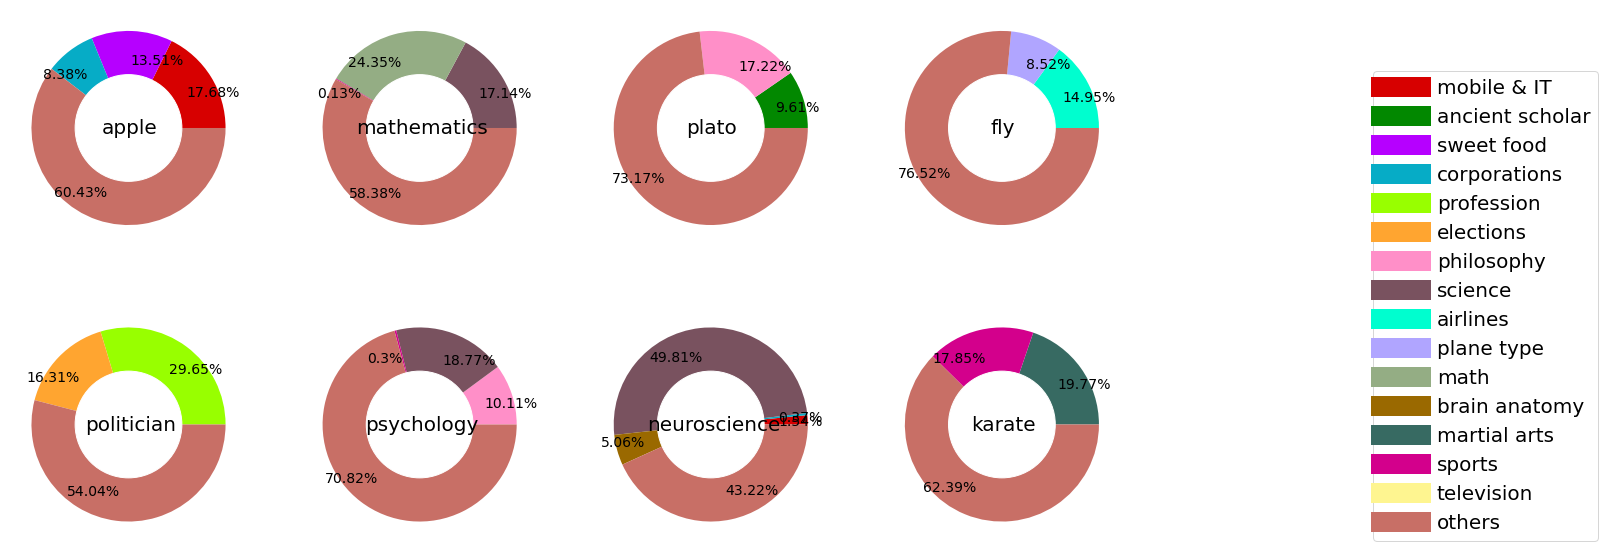
\includegraphics[width=\linewidth]{decomp.png} % Figure image
	\caption{Word vectors can be decomposed into a sparse linear combination of word factors.} % Figure caption
	\label{fig:decomp} % Label for referencing with \ref{bear}
\end{figure*}

In Figure ~\ref{fig:act} there is a table containing a few chosen word factors along with top-activation words. We can see that words are grouped into interpretable, semantically, or syntactically related clusters. 

\begin{figure*}
	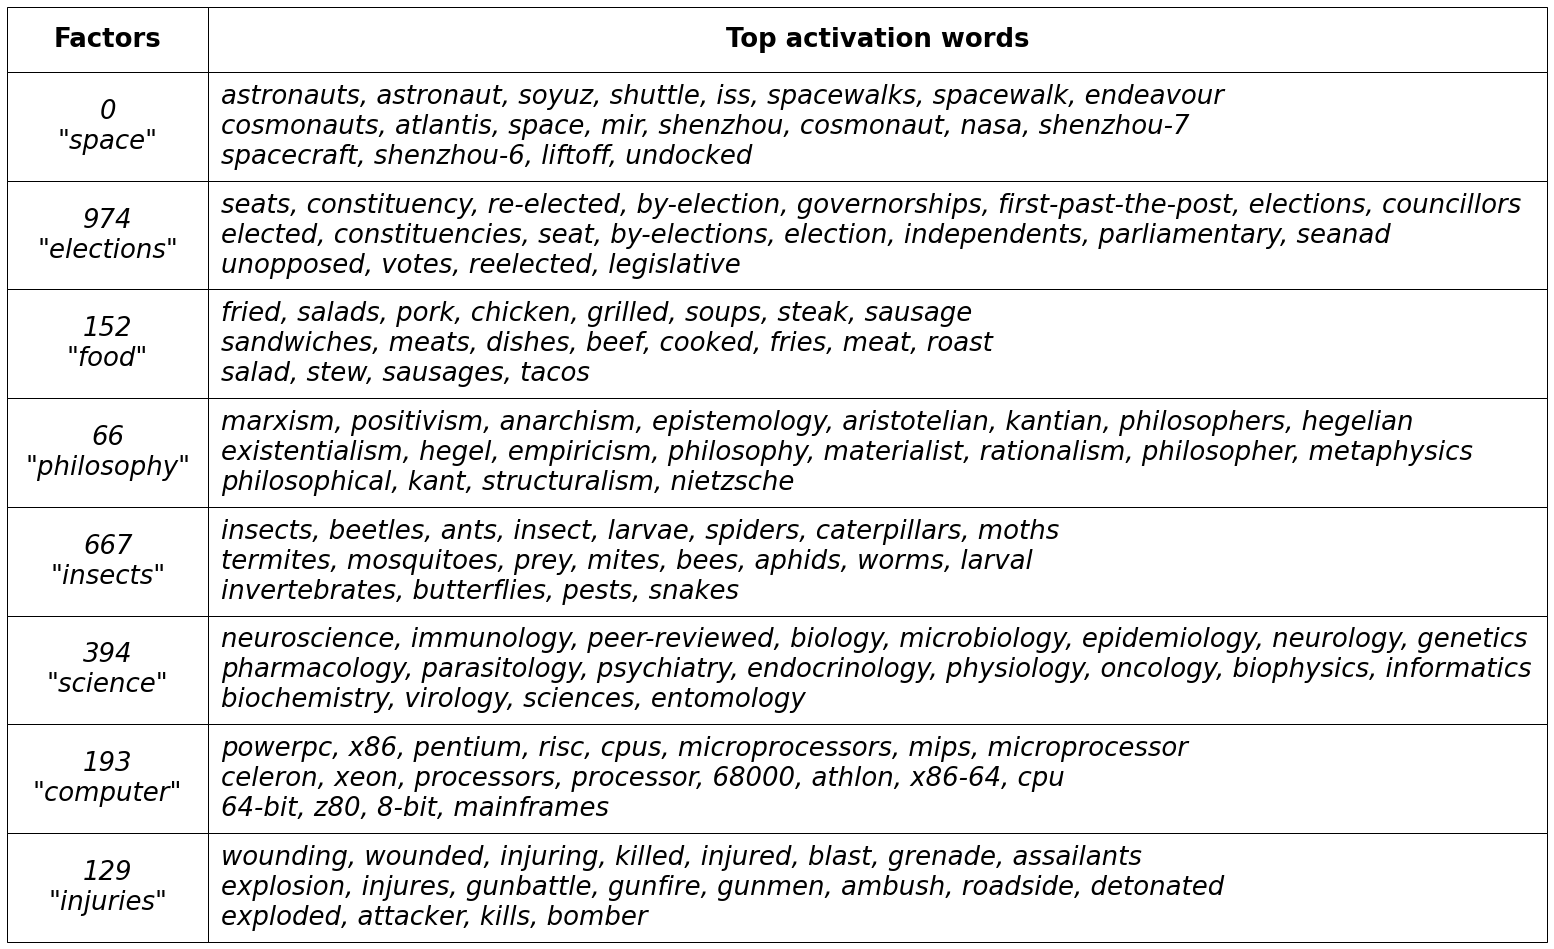
\includegraphics[width=\linewidth]{act_table.png} % Figure image
	\caption{Set of learned factors with its top-activation words. Factors were named manually.} % Figure caption
	\label{fig:act} % Label for referencing with \ref{bear}
\end{figure*}

By adding particular word factors into GloVe word embeddings we can perform interesting manipulations, transforming vectors in a predictable and desirable way (Figure ~\ref{fig:manip}). 

\begin{figure}
	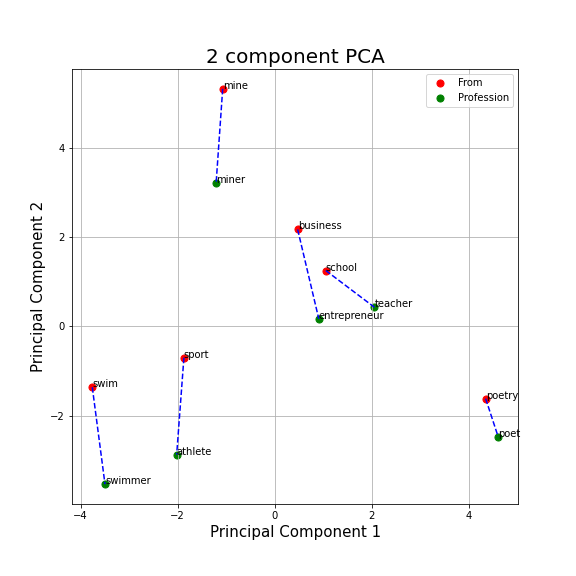
\includegraphics[width=\linewidth]{pca_profession.png} % Figure image
	\caption{PCA visualization of a word analogy
task: “profession”, which can be automatically generated
by the “profession” word factor.} % Figure caption
	\label{fig:pca} % Label for referencing with \ref{bear}
\end{figure}

\begin{table}
	\caption{Vector-factor manipulations. The word vectors’ average norm is $6.9$. The learned word factors all have unit norm. Note that $2nd$ not $1st$ nearest neigbors are displayed.}
	\centering
    \begin{tabular}{|c|c|}	
    \hline
    \textbf{Manipulations} & \textbf{2nd Nearest Neighbor} \\ \hline
    $V_{swim} + 5F_{profession}$ & $V_{swimmer}$ \\ \hline
	$V_{mine} + 5F_{profession}$ & $V_{miner}$ \\ \hline
	$V_{school} + 5F_{profession}$ & $V_{teacher}$ \\ \hline
	$V_{sport} + 5F_{profession}$ & $V_{athlete}$ \\ \hline
    \end{tabular}
    \label{fig:manip}
\end{table}

Figure ~\ref{fig:pro} and Figure ~\ref{fig:ing} show different levels of activation of specified word factors in pairs of words that are syntactically related in the same way. We can see that word factor activations reflect this difference.


\begin{figure}
	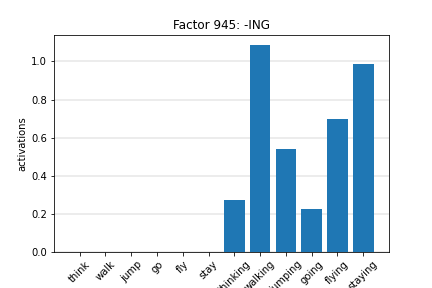
\includegraphics[width=\linewidth]{-ing_factor.png} % Figure image
	\caption{“-ing” factor’s activation w.r.t. a selected set of words contain verbs in basic form and its present continous tense} % Figure caption
	\label{fig:ing} % Label for referencing with \ref{bear}
\end{figure}

\begin{figure}
	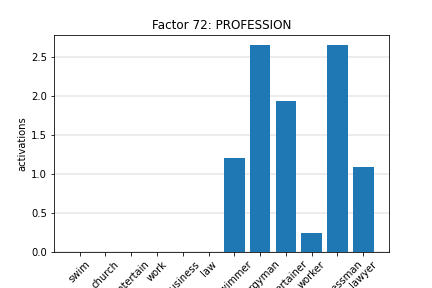
\includegraphics[width=\linewidth]{profession_factor.png} % Figure image
	\caption{“profession” factor’s activation w.r.t. a selected set of words contain action-related words and
their profession form.} % Figure caption
	\label{fig:pro} % Label for referencing with \ref{bear}
\end{figure}

%------------------------------------------------

\section{Conclusions}

Results obtained in this project show that sparse dictionary learning can extract elementary factors from dense, continuous word vectors. By using the learned factors, we can meaningfully decompose or open, otherwise hard to interpret, word vectors and visualize them in many interesting ways. It can guide our intuition and help in better understanding their inner workings and also maybe give some hints in cases when they don’t work as expected, e.g. in word analogy tasks. 

It is interesting to see that word vectors can be thought of, at least to some extent, as a linear combination of word factors that contain often clear semantic or syntactic meaning and that this linear structure emerges from unsupervised learning based on co-occurrence statistics.

This project can be expanded in several ways and directions. One would be performing some form of clustering on learned word factors because it seems that always a few different word factors share similar meanings and could be group together. This could allow for even better, more robust, and complete visualizations. A natural extension of this project would be to apply the same technique on polish word embeddings to see how it would perform in this setting, having in mind that it is much more morphologically rich language. Another interesting direction would be to try to apply sparse dictionary learning to contextual word embeddings like ones produced by BERT or GPT-2 models. 

In summary, sparse dictionary learning is an interesting visualization technique that can be used to open up dense, continuous word embeddings holding potential in developing our understanding of, otherwise hard to interpret, word representations.


\end{document}
